\documentclass[11pt,a4paper]{article}

% --------------------------------------
% Packages
% --------------------------------------
\usepackage[utf8]{inputenc}
\usepackage[T1]{fontenc}
\usepackage{lmodern}
\usepackage{geometry}
\geometry{margin=1in}
\usepackage{microtype}
\usepackage{amsmath, amssymb}
\usepackage{graphicx}
\usepackage{hyperref}
\usepackage{xcolor}
\usepackage{tikz}
\usetikzlibrary{arrows.meta,positioning,shapes}
\usepackage{enumitem}

\hypersetup{
  colorlinks=true,
  linkcolor=blue,
  urlcolor=blue,
  citecolor=blue
}

% --------------------------------------
% Metadata
% --------------------------------------
\title{\textbf{Autonomous Interdependence:\\The Two Axes of Viable Freedom}}
\author{Albert Jan van Hoek \\ \small Evolution by Emergence Project}
\date{\today}

% --------------------------------------
% Document
% --------------------------------------
\begin{document}
\maketitle

\begin{abstract}
Freedom is often conflated with independence---the ability to act without constraint.
Yet complete independence is ecologically, socially, and biologically impossible.
Every living system depends on exchanges with others to stay viable.
This paper introduces a dual-axis model of freedom---\emph{autonomy} and \emph{interdependence}---as complementary properties of viable systems.
Together they yield \textbf{autonomous interdependence}: individual agents who self-regulate while remaining reliably coupled to others.

We formalize this using viability theory: $V_i = f(A_i, \sum_j C_{ij})$ where autonomy $A_i$ and coupling $C_{ij}$ must both exceed minimum thresholds. The multiplicative form $V_i \propto (A_i/A_{\min})^{\alpha_A} \prod_j (C_{ij}/C_{\min})^{\alpha_{ij}}$ captures non-substitutability: deficits in either dimension collapse viability.

This principle clarifies the paradox of freedom (absolute freedom destroys its conditions), resolves the tension between self-determination and social embeddedness, and provides a generalizable framework for stability across scales (persons, institutions, ecologies, and AI networks). We show how stress threatens both axes, how naming fear preserves integrity, and how the framework grounds relational ethics in structural necessity rather than moral preference.
\end{abstract}

\noindent\textbf{Keywords:} autonomy, interdependence, freedom, viability, emergence, networks, trust, repair, relational ethics

\section{The Paradox of Freedom}

In contemporary discourse, \emph{freedom} is often treated as \emph{doing what I want}.
Pursued in the absolute, one person's freedom quickly becomes another's constraint.
At scale this produces polarization, brittle institutions, and ecological overshoot.
\emph{The paradox:} the pursuit of absolute freedom destroys the conditions that make freedom possible.

Traditional theories frame freedom along a single axis---Berlin's negative liberty (freedom \emph{from} interference) versus positive liberty (freedom \emph{to} pursue self-realization)---but this one-dimensional view obscures a deeper structure. A viable account of freedom must include relationship, not only agency.

\section{Freedom as a Dual-Dimensional Construct}

We propose freedom has two orthogonal dimensions:
\begin{itemize}
    \item \textbf{Autonomy} (local): the capacity for self-regulation---to maintain internal stability and act in line with one's values under real constraints.
    \item \textbf{Interdependence} (relational): the capacity for reliable coupling---to exchange information, care, and resources with other autonomous agents.
\end{itemize}

\noindent Failure modes when isolated:
\begin{itemize}
    \item \textbf{Without autonomy:} dependence (loss of self-regulation). \textbf{With inflated autonomy:} isolation (loss of feedback).
    \item \textbf{Without interdependence:} fragmentation (no reciprocity). \textbf{With unbalanced interdependence:} co-dependence or domination.
\end{itemize}

\paragraph{Definition (informal).}
\emph{Autonomous interdependence} is the state in which autonomous agents remain reliably coupled so that each agent's choices increase---not reduce---the viable choices of others.

\subsection{The Viable Region}

Figure~\ref{fig:viable-region} illustrates the dual-axis structure. Viable freedom requires both dimensions to exceed minimum thresholds. The green region represents combinations of autonomy and interdependence that sustain long-term viability.

\begin{figure}[h]
\centering
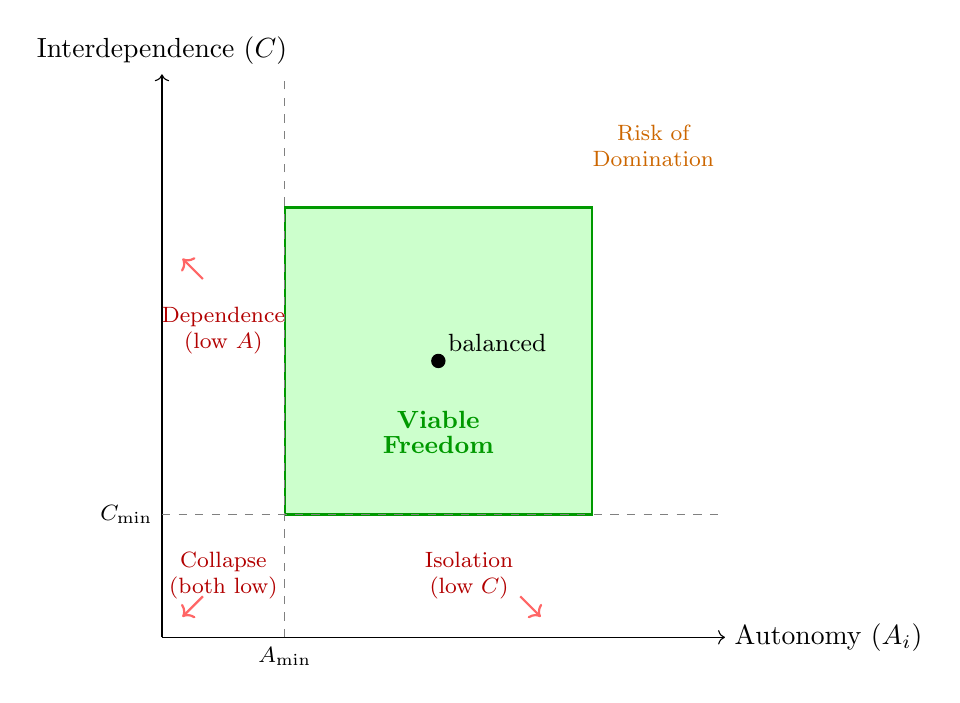
\begin{tikzpicture}[scale=1.3]
    % Axes
    \draw[->] (0,0) -- (5.5,0) node[right]{Autonomy ($A_i$)};
    \draw[->] (0,0) -- (0,5.5) node[above]{Interdependence ($C$)};
    
    % Viable region (green zone)
    \fill[green!20] (1.2,1.2) -- (4.2,1.2) -- (4.2,4.2) -- (1.2,4.2) -- cycle;
    \draw[thick,green!60!black] (1.2,1.2) -- (4.2,1.2) -- (4.2,4.2) -- (1.2,4.2) -- cycle;
    
    % Threshold lines
    \draw[dashed,gray] (1.2,0) -- (1.2,5.5);
    \draw[dashed,gray] (0,1.2) -- (5.5,1.2);
    \node[left,font=\footnotesize] at (0,1.2) {$C_{\min}$};
    \node[below,font=\footnotesize] at (1.2,0) {$A_{\min}$};
    
    % Optimal point
    \fill (2.7,2.7) circle (2pt);
    \node[above right,font=\small] at (2.7,2.7) {balanced};
    
    % Failure zones (labeled with smaller font and better positioning)
    \node[font=\footnotesize,align=center,text=red!70!black] at (0.6,0.6) {Collapse\\(both low)};
    \node[font=\footnotesize,align=center,text=red!70!black] at (0.6,3.0) {Dependence\\(low $A$)};
    \node[font=\footnotesize,align=center,text=red!70!black] at (3.0,0.6) {Isolation\\(low $C$)};
    \node[font=\footnotesize,align=center,text=orange!80!black] at (4.8,4.8) {Risk of\\Domination};
    
    % Viable region label
    \node[font=\small,align=center,color=green!60!black] at (2.7,2.0) {\textbf{Viable}\\[-2pt]\textbf{Freedom}};
    
    % Add small arrows indicating dynamics
    \draw[->,thick,red!60] (0.4,0.4) -- (0.2,0.2);
    \draw[->,thick,red!60] (0.4,3.5) -- (0.2,3.7);
    \draw[->,thick,red!60] (3.5,0.4) -- (3.7,0.2);
\end{tikzpicture}
\caption{The dual-axis structure of freedom. Viable freedom (green) requires both autonomy above $A_{\min}$ (self-regulation capacity) and interdependence above $C_{\min}$ (reliable coupling). Failure modes (red) emerge when either axis is insufficient: collapse when both are low, dependence when only autonomy is deficient, isolation when coupling fails. Arrows indicate trajectories toward failure.}
\label{fig:viable-region}
\end{figure}

\section{Formalization (EbE Framework)}

\subsection{Viability Function}

Let agent $i$ possess internal viability $V_i$ that depends on both internal regulation $A_i$ and relational coupling $C_{ij}$ with others $j$:
\begin{equation}
  V_i = f\!\left(A_i, \sum_{j} C_{ij}\right).
  \label{eq:viability-basic}
\end{equation}

Here, $A_i$ captures internal coherence (self-regulation, adaptive choice, emotional stability) and $C_{ij}$ captures reliability, reciprocity, transparency, and repair capacity in the relationship between $i$ and $j$.

\subsection{Multiplicative Form}

For substrate-dependent systems (cf. ARVC framework~\cite{arvc}), viability can be expressed multiplicatively:
\begin{equation}
  V_i(t) = \left(\frac{A_i(t)}{A_{\min}}\right)^{\alpha_A} \cdot \prod_{j \in \mathcal{N}(i)} \left(\frac{C_{ij}(t)}{C_{\min}}\right)^{\alpha_{ij}}
  \label{eq:viability-multiplicative}
\end{equation}
where $\mathcal{N}(i)$ is $i$'s network neighborhood, and $\alpha$ terms weight relative importance. 

This form ensures $V_i \to 0$ if either autonomy or any critical interdependence falls below threshold---capturing the \emph{non-substitutable} nature of the dual axes. You cannot compensate for lost autonomy with increased interdependence, nor vice versa. This mirrors the multiplicative viability function in substrate theory: $V_I = \prod_k (z^{(k)}/z^{*(k)})^{\alpha_k}$ where violation of any substrate $k$ causes system collapse.

\subsection{Balance Condition}

A system expresses \emph{autonomous interdependence} when
\begin{equation}
  \frac{\partial V_i}{\partial A_i} \approx \frac{\partial V_i}{\partial C_{ij}} \quad \text{for the relevant set of } j,
  \label{eq:balance}
\end{equation}
i.e., when internal and external regulation contribute proportionally to viability. 

Too little coupling ($C \ll C_{\min}$) $\Rightarrow$ isolation collapse; too much coupling relative to autonomy ($C \gg A$) $\Rightarrow$ loss of agency and risk of domination. Sustainable freedom emerges near the balance point where marginal returns to autonomy and interdependence are approximately equal.

\subsection{Connection to Substrate Theory}

In the Attractor-Ratcheted Viability Control (ARVC) framework~\cite{arvc}, systems persist by maintaining substrates $z^{(i)}$ above floors $z^{*(i)}(t)$. We can map:

\begin{itemize}
    \item \textbf{Autonomy} $\leftrightarrow$ capacity to maintain \emph{internal} substrates (cognitive integrity, emotional regulation, decision coherence)
    \item \textbf{Interdependence} $\leftrightarrow$ reliable access to \emph{external} substrates via coupling to others (information, resources, care)
\end{itemize}

The k-cover requirement in ARVC---independent monitors $M_j$ whose collective approval spans all substrates---operationalizes autonomous interdependence:
\begin{itemize}
    \item Each monitor preserves \textbf{autonomy} via independent judgment
    \item Collective approval requirement ensures \textbf{interdependence}
    \item No single point of failure can collapse either dimension
\end{itemize}

This explains why distributed monitoring with heterogeneous incentives (ARVC Assumption 4) preserves freedom: it maintains both local autonomy and global coordination.

\section{Psychological and Societal Implications}

\subsection{Individual Level}

Autonomy is not isolation; it is self-governance \emph{while connected}: emotional regulation, reflective choice, and responsibility for one's own state.
Interdependence then becomes safe exchange between such individuals.
Relationships thrive when partners are both self-stabilizing and mutually responsive.

\textbf{Attachment theory:} Secure attachment in children develops when caregivers provide both (i) scaffolding for autonomy (age-appropriate independence, emotional coaching) and (ii) reliable interdependence (consistent availability, repair after rupture). Anxious attachment reflects low autonomy (over-reliance); avoidant attachment reflects low interdependence (self-sufficiency as defense).

\textbf{Partnership dynamics:} Healthy adult relationships balance differentiation (maintaining separate identities, interests, self-regulation) with integration (shared meaning, coordinated action, mutual support). The failure modes of Figure~\ref{fig:viable-region} manifest as: enmeshment (low autonomy), emotional cut-off (low interdependence), or chronic conflict (oscillation between extremes).

\subsection{Collective Level}

Institutions mirror the same pattern.
Systems fail when either autonomy (local control) or interdependence (shared regulation) dominates unilaterally: centralization squashes local learning and initiative; fragmentation erodes coherence and collective capacity.
Sustainable democracies, ecologies, and AI networks require strong local autonomy \emph{and} reliable global interdependence.

\textbf{Federalism and subsidiarity:} Political systems institutionalize the dual axes through nested autonomy (local control over local matters) and coordinated interdependence (constitutional frameworks, interstate commerce, mutual defense). The principle of subsidiarity---decisions at the lowest viable level---preserves autonomy while preventing race-to-the-bottom dynamics.

\textbf{Commons governance:} Ostrom's principles~\cite{ostrom} for successful commons map onto our framework:
\begin{itemize}
    \item \textbf{Autonomy:} Local rule-making, graduated sanctions, user participation
    \item \textbf{Interdependence:} Monitoring, conflict resolution, nested enterprises
    \item \textbf{Balance:} Recognition of local rights by higher authorities (prevents domination) combined with collective choice arrangements (prevents fragmentation)
\end{itemize}

\section{Freedom Reinterpreted}

We can now define freedom operationally:
\begin{quote}
\textbf{Freedom is the lived capacity to self-regulate while relying on others who reliably self-regulate with you.}
\end{quote}

Freedom is not disconnection; it is \emph{mutual reliability}.
It expands the choice space for all participants, not just one.
In shorthand:
\begin{equation}
  \text{Freedom} \;\propto\; \text{Autonomy} \times \text{Interdependence}.
  \label{eq:freedom-product}
\end{equation}

This formulation resolves several classical tensions:

\textbf{Berlin's two concepts:} Negative liberty (freedom from interference) corresponds to autonomy; positive liberty (freedom to pursue goals) requires interdependence for access to resources and capabilities. The framework shows these are not competing values but complementary dimensions.

\textbf{Individual versus collective:} False dichotomy. Individual autonomy depends on collective interdependence (language, institutions, infrastructure). Collective capacity depends on individual autonomy (distributed intelligence, local adaptation, innovation).

\textbf{Rights versus responsibilities:} Rights protect autonomy (non-interference); responsibilities maintain interdependence (reliability, repair, reciprocity). Both are necessary; neither is sufficient.

\section{Fear, Stress, and the Integrity of Freedom}

\subsection{Fear as Anticipated Substrate Violation}

Fear signals anticipated substrate violation: the agent's world model predicts approaching a viability floor ($z^{(i)} \to z^{*(i)}$). Under stress, two failure modes threaten autonomous interdependence:

\begin{itemize}
    \item \textbf{Autonomy collapse:} Stress degrades self-regulation capacity. The conscious checking loop weakens (cf. consciousness-as-loop framework~\cite{appendixXI}), allowing poorly validated updates to contaminate the world model---\emph{``mud formation.'} Internal coherence $A_i$ declines as decision-making becomes reactive rather than reflective.
    
    \item \textbf{Interdependence collapse:} Fear-driven behaviors (withdrawal, aggression, deception) sever reliable coupling. Signals to others become unreliable; trust erodes. Coupling quality $C_{ij}$ declines as predictability and repair capacity are lost.
\end{itemize}

Importantly, these failures can cascade: autonomy collapse makes one an unreliable partner (degrading others' interdependence); interdependence collapse removes external stabilization (degrading one's own autonomy). This is why stress, left unmanaged, often spirals.

\subsection{Naming Fear: Meta-Model Awareness}

\emph{Naming fear converts it from a driver into data.} When agents recognize ``I am in a stress state,'' they can engage meta-cognitive processes that preserve both axes:

\begin{enumerate}
    \item \textbf{Gate internal updates:} Raise evidence thresholds; slow belief revision; preserve model integrity (preserving $A_i$). This is the ``cognitive hygiene'' mechanism: under detected stress, increase $\phi_t$ (cycle budget) to maintain learning loop quality~\cite{arvc}.
    
    \item \textbf{Signal to others:} Explicitly communicate stress state; request scaffolding; maintain coupling despite internal turbulence (preserving $C_{ij}$). Vulnerability as information rather than weakness.
    
    \item \textbf{Seek stabilizing feedback:} Draw on interdependence to restore autonomy; use reliable others as external regulators during temporary autonomy deficit. Mutual aid as viability strategy.
\end{enumerate}

This meta-awareness is itself a higher-order manifestation of autonomous interdependence: autonomy includes the capacity to recognize and communicate one's own limitations; interdependence includes the willingness to provide temporary support.

\subsection{The Reciprocal Rescue}

Autonomous interdependence creates a \emph{safety net}: 
\begin{itemize}
    \item When one agent's \textbf{autonomy} falters under stress, \textbf{interdependence} provides temporary external regulation (others scaffold decision-making, provide reality checks, offer emotional co-regulation).
    
    \item When one agent's \textbf{connections} fray, \textbf{autonomy} allows them to re-establish coupling from a stable base (self-soothing creates capacity to reach out; clear internal state enables clear communication).
\end{itemize}

This reciprocal rescue is only possible when \emph{both axes are maintained prophylactically}---you cannot draw on reserves you haven't built. Hence the ethical imperative: maintain your autonomy not only for yourself but as a resource for others; maintain your interdependence not only for instrumental benefit but as insurance against your own future deficits.

\paragraph{Connecting to SCAP.} This is why the Sustainable Collaborative Alignment Protocol (SCAP)~\cite{scap} mandates both bias awareness (preserving autonomy via metacognition, Block B) and repair protocols (preserving interdependence via explicit maintenance, Block E). The cycle budget requirement $\phi_t \geq \phi_{\min}$ ensures resources for this prophylactic maintenance of both dimensions.

\section{Applications Across Scales}

The autonomous interdependence framework applies across nested scales:

\subsection{Individual Relationships}

\textbf{Therapeutic context:} Effective therapy builds both autonomy (insight, self-regulation skills, agency) and interdependence (therapeutic alliance, ability to use relationship for co-regulation). Purely autonomy-focused interventions (e.g., self-help, pure CBT) can leave clients isolated; purely interdependence-focused approaches (e.g., dependency on therapist) undermine self-regulation.

\textbf{Parenting:} Developmental task is progressive handoff of regulation from caregiver to child while maintaining reliable connection. Authoritarian parenting (high interdependence demand, low autonomy support) produces dependence; permissive parenting (high autonomy, low interdependence structure) produces fragmentation; authoritative parenting balances both.

\subsection{Organizational Dynamics}

\textbf{Team performance:} High-performing teams exhibit strong role autonomy (members trusted to self-organize within domains, psychological safety for dissent) and rich interdependence (frequent information exchange, shared mental models, rapid conflict repair). Traditional hierarchies overweight interdependence (control) at the expense of autonomy; pure markets overweight autonomy at the expense of coordination.

\textbf{Subsidiarity principle:} Organizations thrive when decision-making occurs at the lowest viable level (preserving autonomy and local knowledge) while maintaining coordination mechanisms for externalities and shared resources (preserving interdependence). Centralization destroys autonomy; balkanization destroys interdependence.

\subsection{Policy and Governance}

\textbf{Democratic resilience:} Healthy democracies balance local autonomy (states' rights, municipal authority, civil society) with national interdependence (constitutional framework, interstate commerce, civil rights enforcement). The failure modes:
\begin{itemize}
    \item \textbf{Authoritarianism:} High centralized control (interdependence without autonomy) $\to$ dependence, lack of local adaptation
    \item \textbf{Failed states:} Weak central capacity (autonomy without interdependence) $\to$ fragmentation, warlordism
    \item \textbf{Polarization:} Oscillation between centralization and fragmentation as neither axis is stable
\end{itemize}

\textbf{International order:} Westphalian sovereignty (national autonomy) combined with international law, trade agreements, and multilateral institutions (interdependence) creates viable global order. Hegemony collapses autonomy; pure anarchy collapses interdependence.

\subsection{Ecological Systems}

\textbf{Species autonomy:} Each species maintains internal regulation (homeostasis, behavioral repertoire, genetic integrity) while embedded in interdependent food webs and nutrient cycles. Invasive species often disrupt by being ``too autonomous'' (lacking natural predators/parasites that couple them to local ecology).

\textbf{Ecosystem services:} Biodiversity provides both autonomy (species can respond independently to local conditions) and interdependence (functional redundancy, trophic cascades that stabilize the whole). Monocultures are low-autonomy (all respond identically to threats); fragmented habitats are low-interdependence (loss of cross-ecosystem flows).

\subsection{AI Multi-Agent Systems}

\textbf{Alignment:} Agent $i$ maintains autonomy via local objective function, internal world model, and capacity for independent judgment. Interdependence via communication protocols, shared state representations, and mutual legibility enables coordination without centralized control.

\textbf{Safety via k-cover:} ARVC's k-cover requirement~\cite{arvc} operationalizes autonomous interdependence in AI governance:
\begin{itemize}
    \item Each monitor $M_j$ preserves \textbf{autonomy}: independent judgment, heterogeneous incentives (Assumption 4), local observables (partial observability)
    \item Collective requirement preserves \textbf{interdependence}: action executes only when monitors spanning all substrates approve
    \item Result: distributed safety enforcement without single point of control or failure
\end{itemize}

This framework suggests that safe AI is not maximally autonomous (unilateral action) nor maximally controlled (centralized authority), but \emph{autonomously interdependent}: local intelligence with distributed oversight.

\section{Ethical Consequences}

This framework yields practical design commitments:
\begin{enumerate}
    \item \textbf{Education}: Train autonomy (self-reflection, self-regulation, metacognition) \emph{before} demanding cooperation. Children need secure base from which to explore; adults need self-knowledge before healthy interdependence.
    
    \item \textbf{Governance}: Build interdependence through transparency, explicit commitments, and repair protocols. Institutions require both checks and balances (autonomy) and coordination mechanisms (interdependence).
    
    \item \textbf{Technology}: Design AI and digital systems that preserve local autonomy while enabling cooperative feedback. Avoid architectures that force choice between control and chaos.
    
    \item \textbf{Relationships}: Evaluate health by \emph{reciprocal viability} rather than simple dependence/independence. Healthy relationships expand both partners' option spaces.
    
    \item \textbf{Conflict resolution}: Recognize that conflicts often stem from unbalanced development along one axis. Solutions require restoring both dimensions, not choosing between them.
\end{enumerate}

\paragraph{From moral preference to structural necessity.}
Crucially, this framework grounds ethics in viability constraints rather than moral axioms. Cooperation is not altruism but enlightened self-interest: your viable freedom depends on others' viable freedom. Defection may yield short-term gains but undermines the interdependence that sustains your own autonomy. This is \emph{forced free will}~\cite{ebe}: you're free to choose, but the space of sustainable choices is structurally constrained by substrate dependencies.

\section{Summary Table}

\begin{center}
\begin{tabular}{|l|p{5.5cm}|p{6cm}|}
\hline
\textbf{Concept} & \textbf{Key property} & \textbf{Failure when isolated} \\ \hline
Autonomy & Self-regulation and agency; capacity to maintain internal substrates & \textbf{Too low:} dependence, loss of self-direction. \textbf{Too high (without C):} isolation, loss of feedback \\ \hline
Interdependence & Reliable reciprocity (transparent, repairable); access to external substrates via coupling & \textbf{Too low:} fragmentation, no mutual support. \textbf{Too high (without A):} co-dependence or domination \\ \hline
Freedom & Viability across both axes; $V_i \propto A_i \times C_{ij}$ & Fragility via loss of feedback (either axis) or collapse (both axes) \\ \hline
Fear & Anticipated substrate violation; signal to raise thresholds & Collapses both axes if unnamed; becomes data if integrated \\ \hline
\end{tabular}
\end{center}

\section{Comparison with Existing Frameworks}

\begin{center}
\small
\begin{tabular}{|l|p{4cm}|p{7cm}|}
\hline
\textbf{Framework} & \textbf{View of Freedom} & \textbf{Limitation / How We Extend} \\ \hline
Berlin's Two Concepts~\cite{berlin} & Negative (freedom from) vs. Positive (freedom to) & Treats as competing; we show they're orthogonal dimensions both necessary \\ \hline
Relational Autonomy~\cite{mackenzie} & Autonomy is socially constituted & Affirms interdependence but lacks formalization; we add viability constraints \\ \hline
Pettit's Republicanism~\cite{pettit} & Freedom as non-domination & Focuses on interdependence axis (preventing domination); we add autonomy requirement \\ \hline
Ostrom's Commons~\cite{ostrom} & Governance requires both local and collective choice & Implicit dual structure; we make it explicit and generalizable \\ \hline
ARVC/SCAP~\cite{arvc,scap} & Viability via substrate maintenance & Technical framework; we provide ethical interpretation \\ \hline
\end{tabular}
\end{center}

\section{Testable Implications}

The framework generates empirically testable predictions:

\paragraph{H1 (Individual well-being).} Life satisfaction correlates with balanced development of both autonomy (locus of control, self-efficacy) and interdependence (social support, relationship quality), not with either alone.

\paragraph{H2 (Relationship stability).} Partnerships show greater stability and satisfaction when both partners score high on autonomy \emph{and} interdependence measures compared to high-on-one-dimension pairs.

\paragraph{H3 (Organizational performance).} Teams with balanced autonomy (role clarity, psychological safety) and interdependence (communication frequency, conflict resolution) outperform teams optimizing either dimension alone.

\paragraph{H4 (Institutional resilience).} Political systems with constitutional protections for local autonomy \emph{and} strong coordinating institutions show greater resilience to shocks than systems tilted toward centralization or fragmentation.

\paragraph{H5 (AI safety).} Multi-agent systems with k-cover requirements (distributed autonomy + coordinated interdependence) maintain safety bounds under perturbations where either pure hierarchical control or pure autonomy fails.

\section{Closing Thought}

True freedom is not the absence of constraints, but the presence of reliable others within them---the equilibrium between self and system: autonomy alive inside interdependence.

This paper has shown that:
\begin{itemize}
    \item Freedom requires \emph{both} autonomy and interdependence, not a choice between them
    \item These dimensions are formally non-substitutable: $V_i \to 0$ if either falls below threshold
    \item The framework applies across scales from individuals to institutions to AI systems
    \item Ethics grounded in viability constraints rather than moral axioms
    \item Cooperation as enlightened self-interest, not altruism
\end{itemize}

The path forward is not maximizing either dimension, but maintaining both in dynamic balance. This requires:
\begin{itemize}
    \item \textbf{Prophylactic maintenance:} Build reserves in both dimensions before crisis
    \item \textbf{Meta-awareness:} Recognize stress and gate updates to preserve integrity
    \item \textbf{Reciprocal rescue:} Draw on interdependence when autonomy falters; draw on autonomy when coupling frays
    \item \textbf{Institutional design:} Create structures that preserve both axes simultaneously
\end{itemize}

The mathematics of viability proves this is possible. The ethics of autonomous interdependence shows why it's necessary. What remains is implementation---the ongoing work of building systems, relationships, and institutions that honor both dimensions of freedom.

\section*{Acknowledgments}

This work builds on the ARVC, SCAP, and EbE frameworks developed as part of the Evolution by Emergence project. Thanks to collaborators who pressure-tested these ideas across disciplines.

\section*{References}

\begin{itemize}[leftmargin=*,label={}]

\item[\textbf{[ARVC]}] van Hoek, A.J. (2025). \emph{Attractor-Ratcheted Viability Control (ARVC) and the Sustainable Collaborative Alignment Protocol (SCAP)}. Evolution by Emergence Project.

\item[\textbf{[SCAP]}] van Hoek, A.J. (2025). \emph{Sustainable Collaborative Alignment Protocol: Logical Premises and Conclusions}. Evolution by Emergence Project, Appendix I.

\item[\textbf{[EbE]}] van Hoek, A.J. (2025). \emph{Evolution by Emergence: A New Paradigm}. Evolution by Emergence Project.

\item[\textbf{[AppendixXI]}] van Hoek, A.J. (2025). \emph{Consciousness as a Checking Loop: Theory and Implications}. Evolution by Emergence Project, Appendix XI.

\item[\textbf{[Berlin]}] Berlin, I. (1969). \emph{Two Concepts of Liberty}. In \emph{Four Essays on Liberty}. Oxford University Press.

\item[\textbf{[Mackenzie]}] Mackenzie, C., \& Stoljar, N. (Eds.). (2000). \emph{Relational Autonomy: Feminist Perspectives on Autonomy, Agency, and the Social Self}. Oxford University Press.

\item[\textbf{[Nedelsky]}] Nedelsky, J. (2011). \emph{Law's Relations: A Relational Theory of Self, Autonomy, and Law}. Oxford University Press.

\item[\textbf{[Ostrom]}] Ostrom, E. (1990). \emph{Governing the Commons: The Evolution of Institutions for Collective Action}. Cambridge University Press.

\item[\textbf{[Pettit]}] Pettit, P. (1997). \emph{Republicanism: A Theory of Freedom and Government}. Oxford University Press.

\end{itemize}

\vspace{1em}
\noindent\textit{Suggested citation:} van Hoek, A. J. (2025). Autonomous Interdependence: The Two Axes of Viable Freedom. \emph{Evolution by Emergence Project} (version \today).

\end{document}